\section{Painting Detection}

\begin{figure}
    \centering
        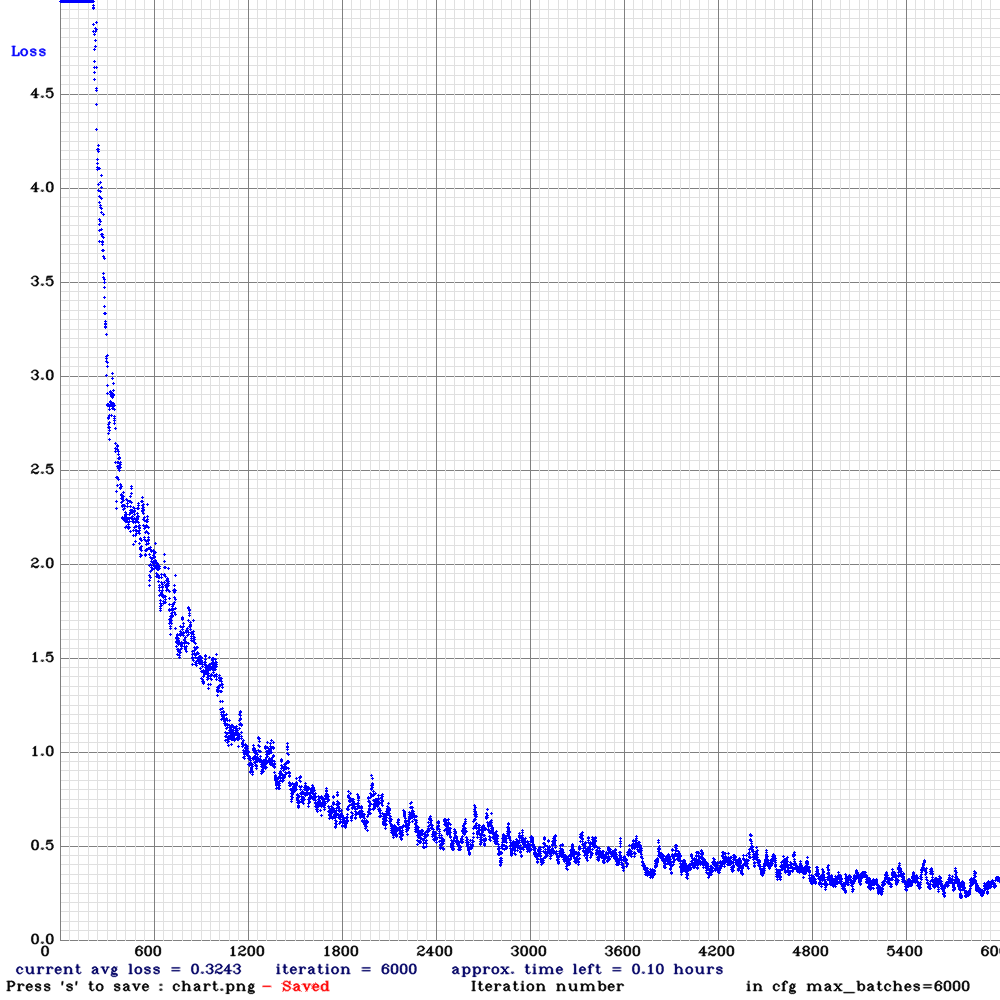
\includegraphics[width=0.4\textwidth]{pictures/painting_detection/chart_.png}
    \caption{This graph represent the train phase of the Neural Network Yolo pre-trained with the dataset Coco and re-trained with our own custom objects, evaluated on the validation set.}
    \label{fig:figura1}
\end{figure}

\begin{figure}
    \centering
        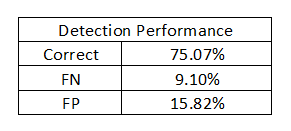
\includegraphics[width=0.4\textwidth]{pictures/painting_detection/tabella1_.png}
    \caption{This chart show the percentage of localization and  errors in the detections for the three categories.}
    \label{fig:figura2}
\end{figure}

\begin{figure}[h] 
    \centering
        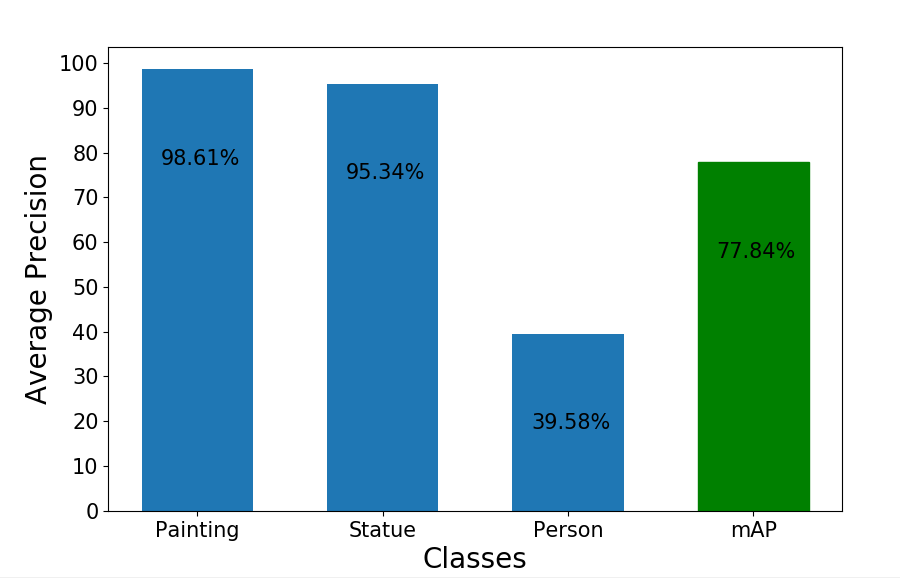
\includegraphics[width=0.45\textwidth]{pictures/painting_detection/performance2.png}
    \caption{Histogram of Average Precision and Mean Average Precision}
    \label{fig:figura3}
\end{figure} 


This part of the system allow the detection of painting and statue through the use of Yolo v4.
Yolo is an architecture that provides a new approach to object detection, a single neural network predicts bounding boxes and class probabilities directly from full images in one evaluation. The version that has been used in this project is the last, released in the april 2020.
In order to use this neural network have been recovered and labeled 1344 images, 1000 of them have been used to train the network, 172 for the validation set and 172 for the test set, providing a total number of 3733 labels. The images of paintings and statues were taken frame by frame by some videos that have been recorded in the Galleria Estense, they have been labeled with the Yolo tool and have been saved in Yolo format. For the class person was instead used a mix of handcrafted label given by the previous video and a small part belonging to another dataset which included people in a museum.

The graph shown in Figure \ref{fig:figura1} illustrates the progress of the test phase in which, every 1000 iterations, has been computed the mAP in the valid set;this was done to take the best weights result which wasn't affected by overfitting.
This approach has allowed to achieve high performance (see Figure \ref{fig:figura2}) %(AP=98.61\% for the class 'painting ', AP = 95.34\% for the class 'statue', AP = 34.08\% for the class 'person' and a final recall of 93.97\%). 
and has also provided a system capable to have many different applications with a good generalization.


\subsection{Comparison with previous technique} 
In a previous pipeline the task of detection was produced in another way.
The system was focused on three main phases: in the first phase the frame which belonged from the video was preprocessed and the edges were computed, then a function had the task of finding the contour of the object and with these contours were detected the region of interest. Despite this method worked well in the main scenery, it hasn't the capability to adapt to strong luminance variation and it wasn't able to manage very well the presence of shadows.
The accuracy that was produced didn't satisfy the standard of the project, for this reason the pipeline was updated.

